
\subsection{Data Processing and Methods}\label{subsection_data_processing_and_methods}

All data processing was performed using the Python programming language, and more specifically the Pandas library, the notebooks used are all available with this paper. Most processing can be separated into categories:

\begin{itemize}

    \item \textbf{Cleaning and Standardizing:} This involves standardizing column names to enable propper merging and cleaning data points to ensure type consistency. Similar procedures where applied to all merged datasets to ensure all received the same treatment. Additionally, cleaning county names took a significant ammount of time, as naming standards diverged between datasets. This was partially autmated by subsituting regular expressions, but also involved partial cleaning by hand. Data aggregation was necessary for type subsets (cities to counties and months to years) in order to maintain the structural consistency of the data. Aggregation methods where performed on a per-variable basis.

    \item \textbf{Merging:} Once the data is cleaned, all different datasets where merged to form a single dataset. Given most of the work was done in the cleaning stage, this only required a small custom merging operation to left-merge all datasets onto the n\_ibuyers dataset on county, state and year. This is saved under the name ``merged.csv.''

    \item \textbf{Manipulation:} The first manipulation performed on the data is its standardizing. This is saved under ``merged\_std.csv.'' Other manipulations mostly involve data aggregation to display summary statistics.

    \item \textbf{Visualization:} Some plots are created using the matplotlib backend of the Pandas library. 

\end{itemize}

\pagebreak
\subsection{Charts}

\begin{table}[!htb]
    \centering
    \caption{Variable Descriptions}\label{variable_descriptions}
    \begin{tabular}{l|l}
    \hline
        \textbf{regressor\_name} &         \textbf{dataset} \\
    \hline
    \hline
    median\_rooms &  median number of rooms per listed property \\ \hline
    educ\_nohs &  percentage of population with no high school diploma \\ \hline
    white &  percentage of white population \\ \hline
        mean\_cash\_public\_assistance\_income\_dollars &  mean per-capita income from public assistance programs (dollars) \\ \hline
    per\_capita\_income\_dollars &  mean per-capita income from all sources (dollars) \\ \hline
    median\_household\_income\_dollars &  mean household income from all sources (dollars) \\ \hline
    part of educ\_further &  percentage of population with degrees beyond high school \\ \hline
    mean\_retirement\_income\_dollars &  mean per-capita retirement income \\ \hline
        median\_age\_years &  median age (years) \\ \hline
    mean\_travel\_time\_to\_work\_minutes &  mean travel time from home to work \\ \hline
    homeowner\_vacancy\_rate &  homeowner vacancy \\ \hline
    move\_post2010 &  percentage of population who moved to current property after 2010 \\ \hline
    average\_household\_size &  average number of people per household \\ \hline
    english\_prof\_pct &             percent of students proficient in English \\ \hline
    math\_prof\_pct &             percent of students proficient in English \\ \hline
    construction &              total expenditure in construction \\ \hline
    median\_listing\_price &           median property listing price \\ \hline
    median\_square\_feet &           median property size (square feet) \\ \hline
    median\_days\_on\_market &           median days property is listed on market \\ \hline
    nlocal\_ibs &        number of local iBuyers \\ \hline
    ntop\_ibs &        number of top iBuyers \\ \hline
    rnaturalinc &       natural rate of population growth \\ \hline
    rnetmig &         rate of net migration \\ \hline
    popestimate &         population size estimate \\ \hline
    annual\_avg\_emplvl &            annual average employment level \\ \hline
    \end{tabular}
\end{table}

\begin{table}
    \centering
    \caption{Dataset of Origin of Selected Regressors}\label{regressor_origin}
    \begin{tabular}{| l || c |}
    \hline
    regressor\_name &          dataset \\
    \hline
    \hline
    median\_rooms &  characteristics \\ \hline
    educ\_nohs &  characteristics \\ \hline
    white &  characteristics \\ \hline
    mean\_cash\_public\_assistance\_income\_dollars &  characteristics \\ \hline
    per\_capita\_income\_dollars &  characteristics \\ \hline
    median\_household\_income\_dollars &  characteristics \\ \hline
    part of educ\_further &  characteristics \\ \hline
    mean\_retirement\_income\_dollars &  characteristics \\ \hline
    median\_age\_years &  characteristics \\ \hline
    mean\_travel\_time\_to\_work\_minutes &  characteristics \\ \hline
    homeowner\_vacancy\_rate &  characteristics \\ \hline
    move\_post2010 &  characteristics \\ \hline
    average\_household\_size &  characteristics \\ \hline
    english\_prof\_pct &             educ \\ \hline
    math\_prof\_pct &             educ \\ \hline
    construction &              gdp \\ \hline
    median\_listing\_price &           h\_vals \\ \hline
    median\_square\_feet &           h\_vals \\ \hline
    median\_days\_on\_market &           h\_vals \\ \hline
    nlocal\_ibs &        n\_ibuyers \\ \hline
    ntop\_ibs &        n\_ibuyers \\ \hline
    rnaturalinc &         pop\_info \\ \hline
    rnetmig &         pop\_info \\ \hline
    popestimate &         pop\_info \\ \hline
    annual\_avg\_emplvl &            wages \\ \hline
    \end{tabular}
\end{table}

\begin{table}
    \centering
    \caption{General Summary Statistics}
    \label{general_stats}
    \begin{tabular}{|l||r|r|}
        \hline
        &           mean &           std \\
        \hline
        \hline
        \textbf{treatment                                 } &       0.141414 &  3.485583e-01 \\ \hline
        \textbf{median\_listing\_price                      } &  274354.042614 &  1.622369e+05 \\ \hline
        \textbf{median\_days\_on\_market                     } &      78.553030 &  2.345368e+01 \\ \hline
        \textbf{median\_rooms                              } &       5.693813 &  5.329772e-01 \\ \hline
        \textbf{homeowner\_vacancy\_rate                    } &       1.639657 &  1.087029e+00 \\ \hline
        \textbf{mean\_travel\_time\_to\_work\_minutes          } &      25.214646 &  5.247091e+00 \\ \hline
        \textbf{math\_prof\_pct                             } &      46.819991 &  1.281202e+01 \\ \hline
        \textbf{english\_prof\_pct                          } &      51.249663 &  1.155455e+01 \\ \hline
        \textbf{median\_square\_feet                        } &    1827.165404 &  5.912998e+02 \\ \hline
        \textbf{median\_age\_years                          } &      38.617677 &  4.654999e+00 \\ \hline
        \textbf{move\_post2010                             } &      43.302652 &  7.698905e+00 \\ \hline
        \textbf{annual\_avg\_emplvl                         } &  154349.486427 &  2.943917e+05 \\ \hline
        \textbf{median\_household\_income\_dollars           } &   61671.342487 &  1.647529e+04 \\ \hline
        \textbf{per\_capita\_income\_dollars                 } &   31669.158775 &  7.945113e+03 \\ \hline
        \textbf{popestimate                               } &  356319.613952 &  7.038671e+05 \\ \hline
        \textbf{rnaturalinc                               } &       2.533129 &  3.524344e+00 \\ \hline
        \textbf{rnetmig                                   } &       4.029436 &  1.067996e+01 \\ \hline
        \textbf{educ\_nohs                                 } &      23.133649 &  1.455964e+01 \\ \hline
        \textbf{educ\_further                              } &      78.632797 &  4.086123e+01 \\ \hline
        \textbf{average\_household\_size                    } &       2.672629 &  2.430024e-01 \\ \hline
        \textbf{white                                     } &      42.600758 &  4.056286e+01 \\ \hline
        \textbf{mean\_cash\_public\_assistance\_income\_dollars} &    2772.248037 &  1.138819e+03 \\ \hline
        \textbf{construction                              } &  712006.203283 &  1.410527e+06 \\ \hline
        \textbf{mean\_retirement\_income\_dollars            } &   26170.630997 &  5.861282e+03 \\ \hline
    \end{tabular}
\end{table}


\begin{table}
    \centering
    \caption{Treatment/Control Summary Statistics}
    \label{treat_cont_comp}
    \begin{tabular}{|l||r|r|r|}
        \hline
        \textbf{treatment} &          0 &           1 &        All \\
        \hline
        \hline
        \textbf{median\_listing\_price                      } &  262823.15 &   344363.01 &  274354.04 \\ \hline
        \textbf{median\_days\_on\_market                     } &      80.19 &       68.60 &      78.55 \\ \hline
        \textbf{median\_rooms                              } &       5.73 &        5.45 &       5.69 \\ \hline
        \textbf{homeowner\_vacancy\_rate                    } &       1.64 &        1.61 &       1.64 \\ \hline
        \textbf{mean\_travel\_time\_to\_work\_minutes          } &      25.22 &       25.20 &      25.21 \\ \hline
        \textbf{math\_prof\_pct                             } &      47.03 &       45.53 &      46.82 \\ \hline
        \textbf{english\_prof\_pct                          } &      51.57 &       49.29 &      51.25 \\ \hline
        \textbf{median\_square\_feet                        } &    1812.60 &     1915.57 &    1827.17 \\ \hline
        \textbf{median\_age\_years                          } &      38.92 &       36.75 &      38.62 \\ \hline
        \textbf{move\_post2010                             } &      42.60 &       47.55 &      43.30 \\ \hline
        \textbf{annual\_avg\_emplvl                         } &  110745.13 &   419090.23 &  154349.49 \\ \hline
        \textbf{median\_household\_income\_dollars           } &   61437.53 &    63090.91 &   61671.34 \\ \hline
        \textbf{per\_capita\_income\_dollars                 } &   31415.57 &    33208.79 &   31669.16 \\ \hline
        \textbf{popestimate                               } &  267214.26 &   897316.43 &  356319.61 \\ \hline
        \textbf{rnaturalinc                               } &       2.26 &        4.22 &       2.53 \\ \hline
        \textbf{rnetmig                                   } &       4.05 &        3.88 &       4.03 \\ \hline
        \textbf{educ\_nohs                                 } &      23.39 &       21.58 &      23.13 \\ \hline
        \textbf{educ\_further                              } &      78.07 &       82.06 &      78.63 \\ \hline
        \textbf{average\_household\_size                    } &       2.66 &        2.76 &       2.67 \\ \hline
        \textbf{white                                     } &      43.19 &       39.04 &      42.60 \\ \hline
        \textbf{mean\_cash\_public\_assistance\_income\_dollars} &    2720.58 &     3049.60 &    2772.25 \\ \hline
        \textbf{construction                              } &  510128.97 &  1937689.42 &  712006.20 \\ \hline
        \textbf{mean\_retirement\_income\_dollars            } &   25906.35 &    27775.20 &   26170.63 \\ \hline
    \end{tabular}
\end{table}

\begin{table}
    \centering
    \caption{2016/2019 Summary Statistics}
    \label{year_comp}
    \begin{tabular}{|l||r|r|r|}
        \hline
        \textbf{treatment} &          0 &           1 &        All \\
        \hline
        \hline
        \textbf{median\_listing\_price                      } &  262823.15 &   344363.01 &  274354.04 \\ \hline
        \textbf{median\_days\_on\_market                     } &      80.19 &       68.60 &      78.55 \\ \hline
        \textbf{median\_rooms                              } &       5.73 &        5.45 &       5.69 \\ \hline
        \textbf{homeowner\_vacancy\_rate                    } &       1.64 &        1.61 &       1.64 \\ \hline
        \textbf{mean\_travel\_time\_to\_work\_minutes          } &      25.22 &       25.20 &      25.21 \\ \hline
        \textbf{math\_prof\_pct                             } &      47.03 &       45.53 &      46.82 \\ \hline
        \textbf{english\_prof\_pct                          } &      51.57 &       49.29 &      51.25 \\ \hline
        \textbf{median\_square\_feet                        } &    1812.60 &     1915.57 &    1827.17 \\ \hline
        \textbf{median\_age\_years                          } &      38.92 &       36.75 &      38.62 \\ \hline
        \textbf{move\_post2010                             } &      42.60 &       47.55 &      43.30 \\ \hline
        \textbf{annual\_avg\_emplvl                         } &  110745.13 &   419090.23 &  154349.49 \\ \hline
        \textbf{median\_household\_income\_dollars           } &   61437.53 &    63090.91 &   61671.34 \\ \hline
        \textbf{per\_capita\_income\_dollars                 } &   31415.57 &    33208.79 &   31669.16 \\ \hline
        \textbf{popestimate                               } &  267214.26 &   897316.43 &  356319.61 \\ \hline
        \textbf{rnaturalinc                               } &       2.26 &        4.22 &       2.53 \\ \hline
        \textbf{rnetmig                                   } &       4.05 &        3.88 &       4.03 \\ \hline
        \textbf{educ\_nohs                                 } &      23.39 &       21.58 &      23.13 \\ \hline
        \textbf{educ\_further                              } &      78.07 &       82.06 &      78.63 \\ \hline
        \textbf{average\_household\_size                    } &       2.66 &        2.76 &       2.67 \\ \hline
        \textbf{white                                     } &      43.19 &       39.04 &      42.60 \\ \hline
        \textbf{mean\_cash\_public\_assistance\_income\_dollars} &    2720.58 &     3049.60 &    2772.25 \\ \hline
        \textbf{construction                              } &  510128.97 &  1937689.42 &  712006.20 \\ \hline
        \textbf{mean\_retirement\_income\_dollars            } &   25906.35 &    27775.20 &   26170.63 \\ \hline
    \end{tabular} \hline
\end{table}

\clearpage

\subsection{Figures}

\begin{figure*}[h]
    \centering
    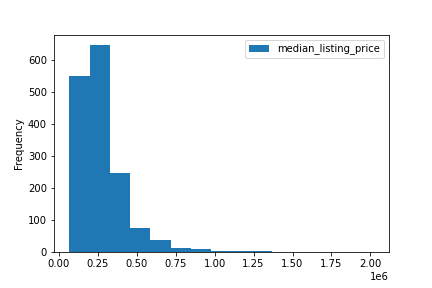
\includegraphics[width=.6\linewidth]{../data_and_processing/media/lst_prc_hist.png}
    \caption{Histogram for Median Listing Price \\ (Aggregate of 2016 and 2019)}
    \label{lst_prc_hist}
\end{figure*}

\begin{figure*}[h]
    \centering
    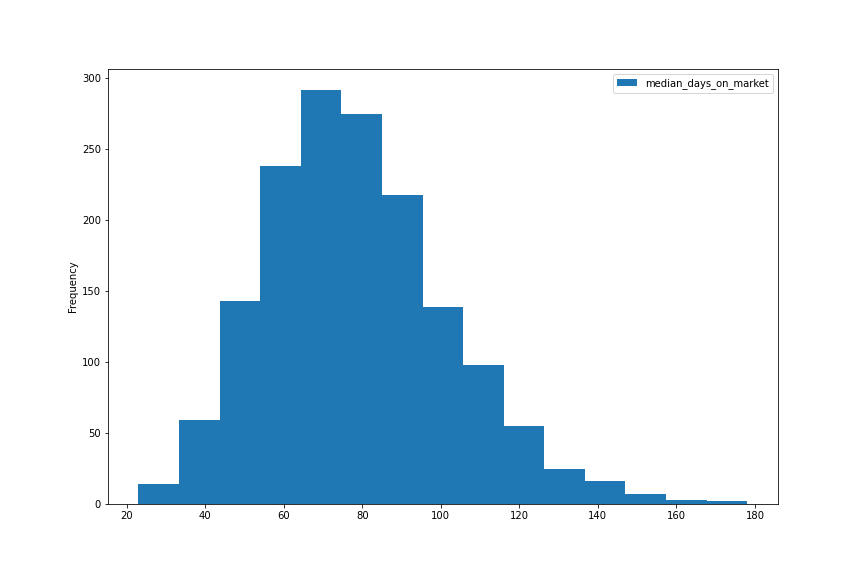
\includegraphics[width=.6\linewidth]{../data_and_processing/media/days_on_mkt_hist.png}
    \caption{Histogram for Median Days on Market \\ (Aggregate of 2016 and 2019)}
    \label{days_on_mkt_hist}
\end{figure*}

\begin{figure}[h]
    \centering
    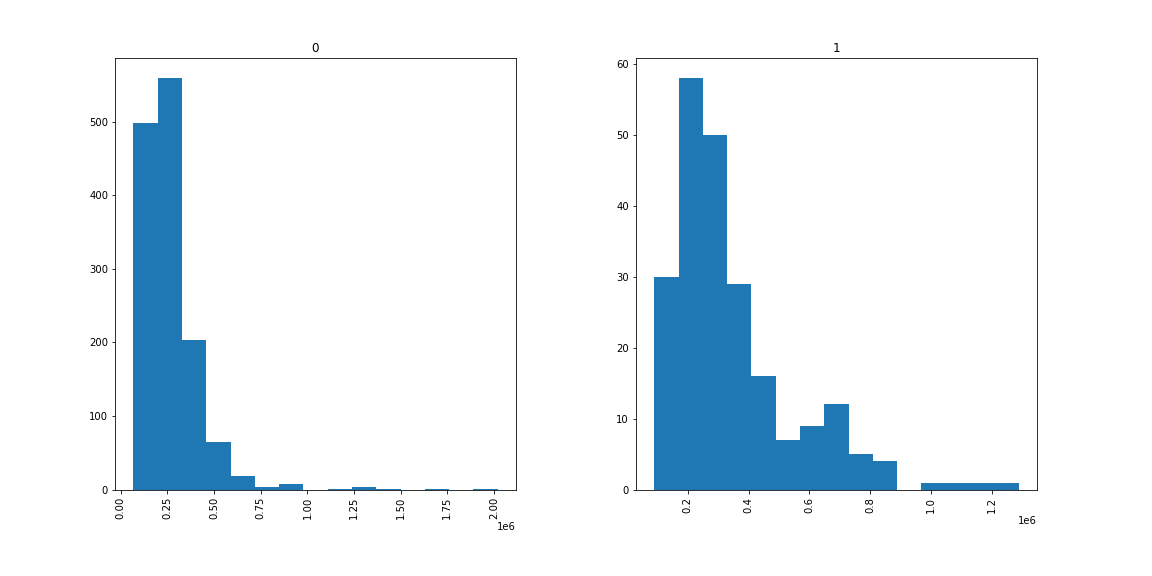
\includegraphics[width=.8\linewidth]{../data_and_processing/media/lst_prc_hist_comp.png}
    \caption{Control/Treatment Comparisson for Median Listing Price}
    \label{lst_prc_hist_comp}
\end{figure}

\begin{figure}[h]
    \centering
    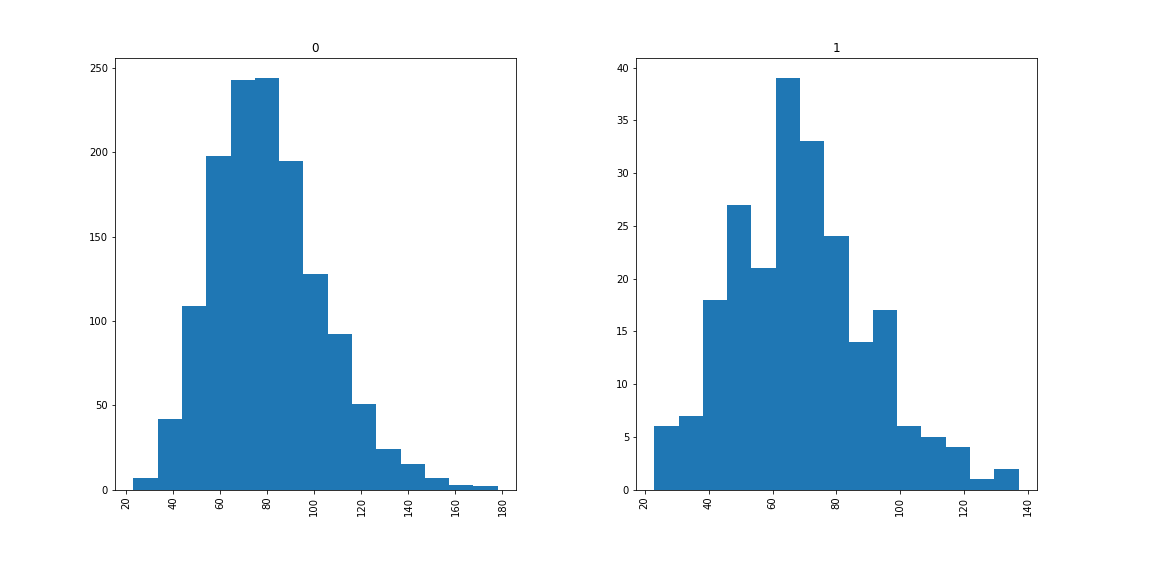
\includegraphics[width=.8\linewidth]{../data_and_processing/media/days_on_mkt_hist_comp.png}
    \caption{Control/Treatment Comparisson for Median Days on Market}
    \label{days_on_mkt_hist_comp}
\end{figure}

\begin{figure}[h]
    \centering
    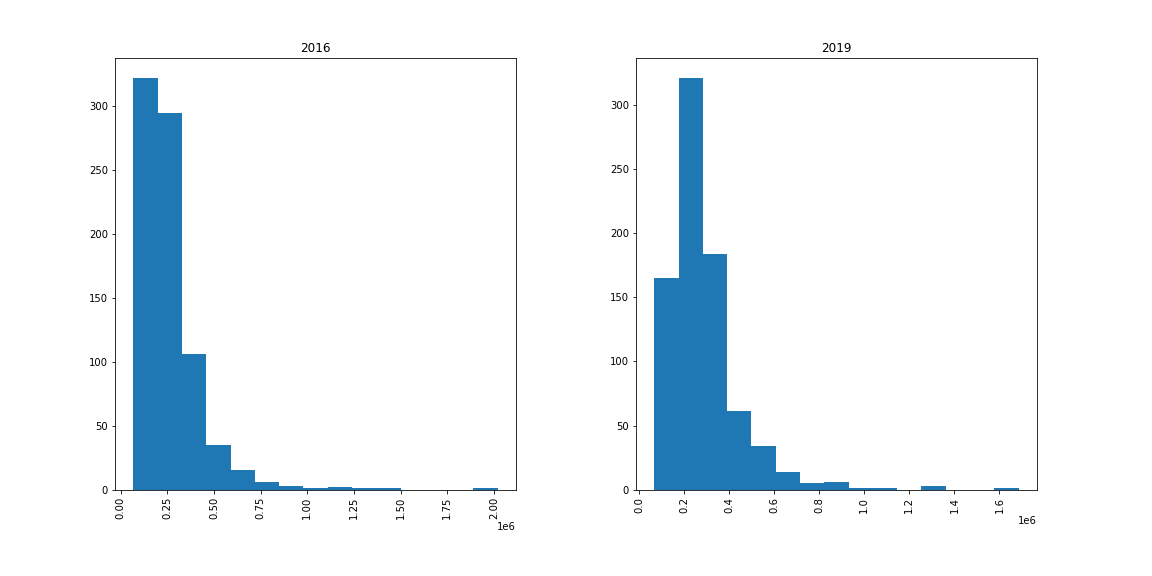
\includegraphics[width=.8\linewidth]{../data_and_processing/media/lst_prc_hist_comp_Y.png}
    \caption{2016/2019 Comparisson for Median Listing Price}
    \label{lst_prc_hist_comp_Y}
\end{figure}

\begin{figure}[h]
    \centering
    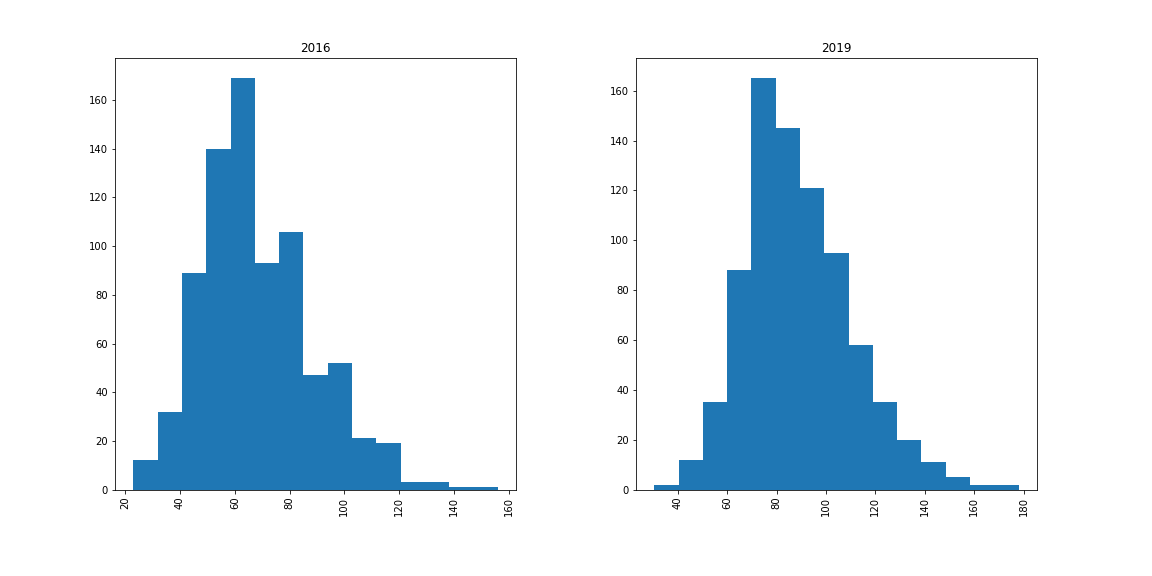
\includegraphics[width=.8\linewidth]{../data_and_processing/media/days_on_mkt_hist_comp_Y.png}
    \caption{2016/2019 Comparisson for Median Days on Market}
    \label{days_on_mkt_hist_comp_Y}
\end{figure}

\begin{figure}[h]
    \centering
    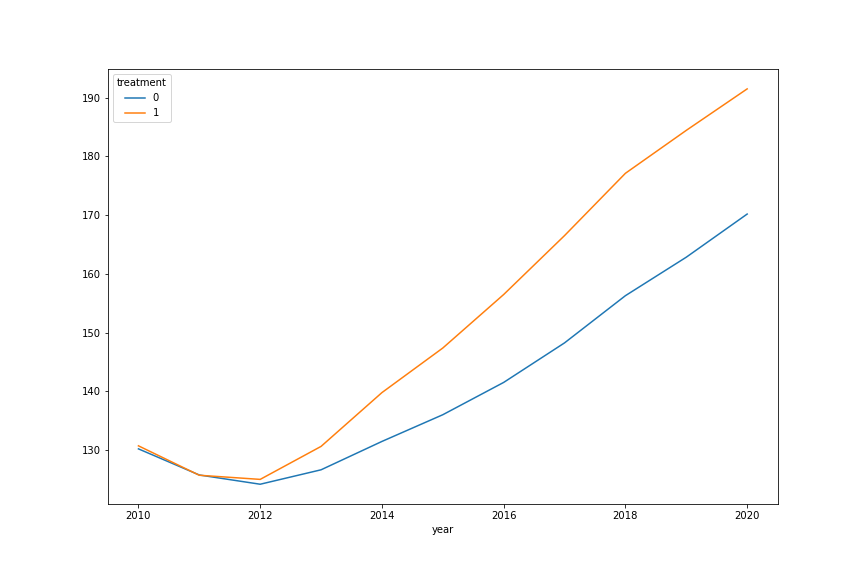
\includegraphics[width=.8\linewidth]{../data_and_processing/media/pta.png}
    \caption{House Price Index Trends for Control and Treatment Data}
    \label{pta}
\end{figure}

\clearpage

\subsection{Difference-In-Difference Results}

Bellow is the results of six difference-in-difference regressions. The columns are as follows:

\begin{enumerate}

    \item Regress listing price on no covariates

    \item Regress time on market on no covariates

    \item Regress listing price on all covariates and number of iBuyers

    \item Regress time on market  on all covariates and number of iBuyers

    \item Regress listing price on all covariates and presence of iBuyers (binary)

    \item Regress time on market on all covariates and presence of iBuyers (binary)

\end{enumerate}


\begingroup
    {
    \small
    \def\sym#1{\ifmmode^{#1}\else\(^{#1}\)\fi}
    \centering
    \begin{longtable}{|l|ll|ll|ll|}
    \caption{Difference-in-Difference Regression Results}
    \label{dd_res}
            \hline\hline
                        &\multicolumn{1}{c}{(1)}&\multicolumn{1}{c}{(2)}&\multicolumn{1}{c}{(3)}&\multicolumn{1}{c}{(4)}&\multicolumn{1}{c}{(5)}&\multicolumn{1}{c}{(6)}\\
                        &\multicolumn{1}{c}{\_\_000001}&\multicolumn{1}{c}{\_\_000001}&\multicolumn{1}{c}{\_\_000001}&\multicolumn{1}{c}{\_\_000001}&\multicolumn{1}{c}{\_\_000001}&\multicolumn{1}{c}{\_\_000001}\\
            \hline
            time        &      0.0992\sym{***}&       21.06\sym{***}&      0.0507         &       25.24\sym{**} &      0.0517         &       25.21\sym{**} \\
                        &      (0.03)         &      (1.12)         &      (0.13)         &      (8.67)         &      (0.13)         &      (8.66)         \\
            [1em]
            treatment   &       0.250\sym{***}&      -9.672\sym{***}&      0.0256         &       0.306         &      0.0257         &       0.325         \\
                        &      (0.05)         &      (2.11)         &      (0.03)         &      (1.82)         &      (0.03)         &      (1.82)         \\
            [1em]
            \_diff       &     -0.0136         &      -3.726         &     0.00969         &      -3.658         &     0.00842         &      -4.337         \\
                        &      (0.07)         &      (2.99)         &      (0.05)         &      (3.10)         &      (0.04)         &      (2.52)         \\
            [1em]
            median\_rooms&                     &                     &      -0.364\sym{***}&      -5.296\sym{***}&      -0.364\sym{***}&      -5.254\sym{***}\\
                        &                     &                     &      (0.02)         &      (1.23)         &      (0.02)         &      (1.23)         \\
            [1em]
            homeowner\_vacancy\_rate&                     &                     &     -0.0245\sym{***}&       3.843\sym{***}&     -0.0246\sym{***}&       3.838\sym{***}\\
                        &                     &                     &      (0.01)         &      (0.45)         &      (0.01)         &      (0.45)         \\
            [1em]
            mean\_travel\_time\_to\_work\_minutes&                     &                     &     0.00478\sym{**} &      -0.301\sym{*}  &     0.00483\sym{**} &      -0.298\sym{*}  \\
                        &                     &                     &      (0.00)         &      (0.12)         &      (0.00)         &      (0.12)         \\
            [1em]
            math\_prof\_pct&                     &                     &    -0.00541\sym{***}&       0.105         &    -0.00545\sym{***}&       0.103         \\
                        &                     &                     &      (0.00)         &      (0.06)         &      (0.00)         &      (0.06)         \\
            [1em]
            english\_prof\_pct&                     &                     &     0.00613\sym{***}&     -0.0158         &     0.00616\sym{***}&     -0.0147         \\
                        &                     &                     &      (0.00)         &      (0.07)         &      (0.00)         &      (0.07)         \\
            [1em]
            median\_square\_feet&                     &                     &    0.000131\sym{***}&   -0.000470         &    0.000131\sym{***}&   -0.000470         \\
                        &                     &                     &      (0.00)         &      (0.00)         &      (0.00)         &      (0.00)         \\
            [1em]
            median\_age\_years&                     &                     &      0.0179\sym{***}&      0.0802         &      0.0179\sym{***}&      0.0758         \\
                        &                     &                     &      (0.00)         &      (0.24)         &      (0.00)         &      (0.24)         \\
            [1em]
            move\_post2010&                     &                     &    -0.00178         &      -1.182\sym{***}&    -0.00177         &      -1.184\sym{***}\\
                        &                     &                     &      (0.00)         &      (0.12)         &      (0.00)         &      (0.12)         \\
            [1em]
            annual\_avg\_emplvl&                     &                     &-0.000000372\sym{***}&  -0.0000194\sym{**} &-0.000000377\sym{***}&  -0.0000195\sym{**} \\
                        &                     &                     &      (0.00)         &      (0.00)         &      (0.00)         &      (0.00)         \\
            [1em]
            median\_household\_income\_dollars&                     &                     &  0.00000877\sym{***}&   -0.000404\sym{***}&  0.00000871\sym{***}&   -0.000410\sym{***}\\
                        &                     &                     &      (0.00)         &      (0.00)         &      (0.00)         &      (0.00)         \\
            [1em]
            per\_capita\_income\_dollars&                     &                     &   0.0000124\sym{***}&  -0.0000133         &   0.0000124\sym{***}& -0.00000532         \\
                        &                     &                     &      (0.00)         &      (0.00)         &      (0.00)         &      (0.00)         \\
            [1em]
            popestimate &                     &                     & 0.000000117\sym{***}&  0.00000327         & 0.000000117\sym{***}&  0.00000329         \\
                        &                     &                     &      (0.00)         &      (0.00)         &      (0.00)         &      (0.00)         \\
            [1em]
            rnaturalinc &                     &                     &      0.0151\sym{**} &     -0.0984         &      0.0152\sym{**} &     -0.0936         \\
                        &                     &                     &      (0.00)         &      (0.32)         &      (0.00)         &      (0.32)         \\
            [1em]
            rnetmig     &                     &                     &     0.00610\sym{***}&     -0.0439         &     0.00610\sym{***}&     -0.0431         \\
                        &                     &                     &      (0.00)         &      (0.06)         &      (0.00)         &      (0.06)         \\
            [1em]
            educ\_nohs   &                     &                     &    -0.00601\sym{***}&       0.145         &    -0.00597\sym{***}&       0.145         \\
                        &                     &                     &      (0.00)         &      (0.11)         &      (0.00)         &      (0.11)         \\
            [1em]
            educ\_further&                     &                     &     0.00375\sym{**} &       0.160         &     0.00380\sym{**} &       0.161         \\
                        &                     &                     &      (0.00)         &      (0.09)         &      (0.00)         &      (0.09)         \\
            [1em]
            average\_household\_size\_of\_owner\_&                     &                     &       0.344\sym{***}&      -4.176         &       0.343\sym{***}&      -4.176         \\
                        &                     &                     &      (0.05)         &      (3.47)         &      (0.05)         &      (3.47)         \\
            [1em]
            white       &                     &                     &    0.000435         &       0.105\sym{*}  &    0.000482         &       0.107\sym{*}  \\
                        &                     &                     &      (0.00)         &      (0.05)         &      (0.00)         &      (0.05)         \\
            [1em]
            mean\_cash\_public\_assistance\_inco&                     &                     &   0.0000248\sym{***}&    -0.00149\sym{***}&   0.0000247\sym{***}&    -0.00149\sym{***}\\
                        &                     &                     &      (0.00)         &      (0.00)         &      (0.00)         &      (0.00)         \\
            [1em]
            construction&                     &                     &    3.33e-08\sym{*}  & 0.000000593         &    3.37e-08\sym{*}  & 0.000000580         \\
                        &                     &                     &      (0.00)         &      (0.00)         &      (0.00)         &      (0.00)         \\
            [1em]
            mean\_retirement\_income\_dollars&                     &                     &   0.0000106\sym{***}&    0.000513\sym{***}&   0.0000106\sym{***}&    0.000515\sym{***}\\
                        &                     &                     &      (0.00)         &      (0.00)         &      (0.00)         &      (0.00)         \\
            [1em]
            ntop\_ibs    &                     &                     &      0.0692         &       1.912         &                     &                     \\
                        &                     &                     &      (0.07)         &      (5.01)         &                     &                     \\
            [1em]
            nlocal\_ibs  &                     &                     &    -0.00116         &      -0.189         &                     &                     \\
                        &                     &                     &      (0.01)         &      (0.44)         &                     &                     \\
            [1em]
            \_cons      &       12.31\sym{***}&       69.60\sym{***}&       12.36\sym{***}&       65.41\sym{***}&       12.36\sym{***}&       65.42\sym{***}\\
                        &      (0.02)         &      (0.80)         &      (0.06)         &      (4.38)         &      (0.06)         &      (4.38)         \\
            \hline
            \(N\)       &        1584         &        1584         &        1397         &        1397         &        1397         &        1397         \\
            \hline\hline
        \multicolumn{7}{l}{\footnotesize Standard errors in parentheses}\\
        \multicolumn{7}{l}{\footnotesize \sym{*} \(p<0.05\), \sym{**} \(p<0.01\), \sym{***} \(p<0.001\)}\\
    \end{longtable}
    }
\endgroup
